\section{Lista 3: Algoritmos Recursivos} % <-----------------------------------------------------------------------------


\subsection{Algoritmo LMF} % <-----------------------------------------------------------------------------
\todo[inline, color=yellow!30]{Organizar}

Podemos inicialmente definir a função erro para esse filtro como

\begin{align}
    e(n) &= d(n) - y(n), \\
    e(n) &= d(n) - \mathbf{w}^{\text{T}}(n)\mathbf{x}(n),
\end{align}

e para obtermos a nova expressão de recurssão precisamos primeiro obter o equacionamento para o vetor gradiente instântaneo de $\mathbb{E}\{e^{4}(n)\}$. Isso pode ser prontamente obtido por meio do auxílio de uma derivação implícita

\begin{align}
    \nabla_{\mathbf{w}} \mathbb{E}\{e^{4}(n)\} &= \frac{\partial \mathbb{E}\{e^{4}(n)\}}{\partial \mathbf{w}} = \mathbb{E}\{ \frac{\partial e^{4}(n)}{\partial \mathbf{w}}\} = \mathbb{E}\{ \frac{\partial e^{4}(n)}{\partial e(n)} \frac{\partial e(n) }{\partial \mathbf{w}}\}, \\
    \nabla_{\mathbf{w}} \mathbb{E}\{e^{4}(n)\} &= \mathbb{E}\{4 e^{3}(n) \frac{\partial (d(n) - \mathbf{w}^{\text{T}}(n)\mathbf{x}(n)) }{\partial \mathbf{w}}\} = \mathbb{E}\{4 e^{3}(n) (0 - \mathbf{x}(n))\}, \\
    \nabla_{\mathbf{w}} \mathbb{E}\{e^{4}(n)\} &= - 4 \mathbb{E}\{e^{3}(n) \mathbf{x}(n)\}.
\end{align}

Desse modo, para que a minimização de $\mathbb{E}\{e^{4}(n)\}$ seja atingida precisamos garantir apenas que o vetor $x(n)$ tenha entradas ortogonais ao vetor erro $e(n)$. Assim, é necessário que a seguinte equação seja verdade

\begin{align}
    \mathbb{E}\{e^{3}(n) \mathbf{x}(n)\} &= 0, \\
    \mathbb{E}\{(d(n) - \mathbf{w}^{\text{T}}(n)\mathbf{x}(n))^{3} \mathbf{x}(n)\} &= 0, 
\end{align}

onde é possível demonstrar que existe convergência em média para essa expressão se definirmos o passo de aprendizado no seguinte intervalo\footnote{A demonstração da propriedade foi extensivamente explicada no artigo \textit{The Least Mean Square Fourth (LMF) Algorithm and Its Family} de 1984 por Eugene Walash e Bernard Widrow.}

\begin{align}
    1 < \mu < \frac{1}{6 \sigma^{2}_{z} \lambda_{\text{max}}},
\end{align}

onde $\sigma^{2}_{z}$ é a variância do ruído presente e $\lambda_{\text{max}}$ é o maior autovalor da matriz de autocorrelação $\mathbf{R}_{x}$. Por fim, a partir dessas observações podemos escrever a expressão de recurssão para o LMF utilizando 
a expressão padrão para o algoritmo do gradiente descendente\footnote{Essa expressão é brevemente introduzida no livro texto da disciplina.}

\begin{align}
    \mathbf{w}(n + 1) &= \mathbf{w}(n) - \mu \mathbf{g}_{w}(n), \\
    \mathbf{w}(n + 1) &= \mathbf{w}(n) + 4 \mu e^{3}(n) \mathbf{x}(n),
\end{align}

onde sabemos que o erro é dado por $e(n) = d(n) - \mathbf{w}^{\text{T}}(n)\mathbf{x}(n)$.
\clearpage


\subsection{Algoritmo LMS} % <-----------------------------------------------------------------------------
\todo[inline, color=yellow!30]{Organizar}
    
\begin{enumerate}
    
    \item a condição para convergência do algoritmo em média.
    
        \textcolor{red}{Solução:}
        
        A condição de convergência está diretamente associada com o erro nos coeficientes do filtro adaptativo para cada iteração.
        Desse modo, podemos iniciar o estudo desse tópico com a seguinte expressão que relaciona o erro dos coeficientes do filtro de um iteração
        $k$ para a solução ótima
        
        \begin{align}
            \Delta \mathbf{w}(n) = \mathbf{w}(n) - \mathbf{w}_{\text{opt}},
        \end{align}

        e assim podemos reescrever a função de recurssão do LMS do seguinte modo

        \begin{align}
            \Delta \mathbf{w}(n + 1) &= \Delta \mathbf{w}(n) + 2 \mu e(n) \mathbf{x}(n), \\
            \Delta \mathbf{w}(n + 1) &= \Delta \mathbf{w}(n) + 2 \mu \mathbf{x}(n) \left[\mathbf{x}^{\text{T}}(n)\mathbf{w}_{\text{opt}} + z(n) - \mathbf{x}^{\text{T}}(n)\mathbf{w}(n)\right], \\
            \Delta \mathbf{w}(n + 1) &= \Delta \mathbf{w}(n) + 2 \mu \mathbf{x}(n) \left[e_{\text{opt}}(n) - \mathbf{x}^{\text{T}}(n) \Delta \mathbf{w}(n)\right], \\
            \Delta \mathbf{w}(n + 1) &= \left[ \mathbf{I} - 2 \mu \mathbf{x}(n) \mathbf{x}^{\text{T}}(n) \right] \Delta \mathbf{w}(n) + 2 \mu e_{\text{opt}}(n) \mathbf{x}(n)
        \end{align}
    
        onde $z(n) \in \mathcal{N}(0,\sigma^{2})$ e $e_{\text{opt}}(n) = z(n)$. Indicando que, para o caso ideal, teríamos que nos preocupar apenas com o erro introduzido pelas componentes ruidosas do sistema.
        Ademais, também utilizamos o fato de que $e(n) = e^{\text{T}}(n) = \mathbf{w}^{\text{T}}_{\text{opt}}\mathbf{x}(n) + z(n) - \mathbf{w}^{\text{T}}(n)\mathbf{x}(n) = \mathbf{x}^{\text{T}}(n)\mathbf{w}_{\text{opt}} + z(n) - \mathbf{x}^{\text{T}}(n)\mathbf{w}(n)$.
        Em sequência, podemos escrever o valor esperado para o erro como

        \begin{align}
            \mathbb{E}\{\Delta \mathbf{w}(n + 1)\} &= \mathbb{E}\{\left[ \mathbf{I} - 2 \mu \mathbf{x}(n) \mathbf{x}^{\text{T}}(n) \right] \Delta \mathbf{w}(n) + 2 \mu e_{\text{opt}}(n) \mathbf{x}(n)\}, \\
            \mathbb{E}\{\Delta \mathbf{w}(n + 1)\} &= \mathbb{E}\{\left[ \mathbf{I} - 2 \mu \mathbf{x}(n) \mathbf{x}^{\text{T}}(n) \right] \Delta \mathbf{w}(n)\} + 2 \mu \mathbb{E}\{e_{\text{opt}}(n) \mathbf{x}(n)\}
        \end{align}
        
        onde utilizamos a propriedade de linearidade do operador valor esperado. Ao assumirmos que $\mathbf{x}(n)$ é simultaneamente ortogonal aos elementos $e_{\text{opt}}(n)$ e $\Delta \mathbf{w}(n)$ podemos simplificar a expressão acima por
        
        \begin{align}
            \mathbb{E}\{\Delta \mathbf{w}(n + 1)\} &= \left[ \mathbf{I} - 2 \mu \mathbb{E}\{\mathbf{x}(n) \mathbf{x}^{\text{T}}(n)\} \right] \mathbb{E}\{\Delta \mathbf{w}(n)\}, \\
            \mathbb{E}\{\Delta \mathbf{w}(n + 1)\} &= \left( \mathbf{I} - 2 \mu \mathbf{R}_{x} \right) \mathbb{E}\{\Delta \mathbf{w}(n)\},
        \end{align}

        onde podemos utilizar a noção de que $\mathbb{E}\{ \mathbf{I} \} = \mathbf{I}$ uma vez que temos um operador linear. Em continuidade, podemos supor que existe uma matriz $\mathbf{Q}$ unitária que diagonaliza $\mathbf{R}_{x}$
        de tal modo que temos 

        \begin{align}
            \mathbb{E}\{ \mathbf{Q}^{\text{T}} \Delta \mathbf{w}(n + 1) \} &= \left( \mathbf{I} - 2 \mu \mathbf{Q}^{\text{T}} \mathbf{R}_{x} \right) \mathbf{I} \mathbb{E}\{ \Delta \mathbf{w}(n)\}, \\
            \mathbb{E}\{ \mathbf{Q}^{\text{T}} \Delta \mathbf{w}(n + 1) \} &= \left( \mathbf{I} - 2 \mu \mathbf{Q}^{\text{T}} \mathbf{R}_{x} \right) \mathbf{Q} \mathbf{Q}^{\text{T}} \mathbb{E}\{ \Delta \mathbf{w}(n)\}, \\
            \mathbb{E}\{ \mathbf{Q}^{\text{T}} \Delta \mathbf{w}(n + 1) \} &= \left( \mathbf{I} - 2 \mu \mathbf{Q}^{\text{T}} \mathbf{R}_{x} \mathbf{Q} \right) \mathbb{E}\{ \mathbf{Q}^{\text{T}} \Delta \mathbf{w}(n)\}, \\
            \mathbb{E}\{\Delta \mathbf{w}'(n + 1)\} &= \left( \mathbf{I} - 2 \mu \mathbf{\Lambda} \right) \mathbb{E}\{\Delta \mathbf{w}'(n)\}.
        \end{align}

        Podemos, por fim, expandir os termos à esquerda e chegar na seguinte expressão para a análise do comportamento de convergência dos coeficientes de filtro

        \begin{align}
            \mathbb{E}\{ \Delta \mathbf{w}'(n + 1) \} &= \left( \mathbf{I} - 2 \mu \mathbf{\Lambda} \right)^{n + 1} \mathbb{E}\{\Delta \mathbf{w}'(0)\}, \\
            \mathbb{E}\{ \Delta \mathbf{w}'(n + 1) \} &= 
            \begin{bmatrix}
                (1 - 2 \mu \lambda_{1})^{n + 1} & 0 & \cdots & 0 \\
                0 & (1 - 2 \mu \lambda_{2})^{n + 1} & \cdots & \vdots \\
                \vdots & \vdots & \ddots & \vdots \\
                0 & 0 & \cdots & (1 - 2 \mu \lambda_{N})^{n + 1}
            \end{bmatrix} 
            \mathbb{E}\{ \Delta \mathbf{w}'(0)\},	
        \end{align}

        onde temos que $\lambda_{n} \forall n \in \{1, \cdots, N\}$ são os autovalores da matriz de autocorrelação. Portanto, vemos que para garantir a estabilidade da convergência é necessário 
        apenas que o passo de aprendizado do algoritmo seja definido pela seguinte inequação

        \begin{align}
            0 < \mu < \frac{1}{\lambda}_{\text{max}},
        \end{align}

        pois desse modo conseguimos garantir que os valores da diagonal irão tender a zero a medida que o número de iterações do algoritmo tende ao infinito. Ademais, é interessante ressaltar que a escolha 
        do valor de $\mu$ deve também levar em consideração o espalhamento de energia da matriz de correlação. Dessa forma, se não há grande diferença entre
        os valores númericos dos autovalores, então seria aconselhável escolher um passo de aprendizado muito menor do que aquele definido pelo limite superior da expressão obtida acima.
        
        \item o erro em excesso em média quadrática. 
    
        \textcolor{red}{Solução:}
        
        O erro em excesso é normalmente ocasionado pelos termos ruidosos presentes no gradiente, impedindo que os coeficientes convirjam de forma exata para a solução ótima. 
        Podemos iniciar essa análise escrevendo a equação para o erro de estimação para um determinado instante $n$ como se segue

        \begin{align}
            e(n) &= d(n) - \mathbf{w}^{\text{T}}_{\text{opt}} \mathbf{x}(n) - \Delta \mathbf{w}^{\text{T}}(n) \mathbf{x}(n), \\
            e(n) &= e_{\text{opt}}(n) - \Delta \mathbf{w}^{\text{T}}(n) \mathbf{x}(n),
        \end{align}

        onde o erro quadrático é expresso por

        \begin{align}
            e^{2}(n) &= e^{2}_{\text{opt}}(n) - 2 e_{\text{opt}}(n) \Delta \mathbf{w}^{\text{T}}(n) \mathbf{x}(n) + \Delta \mathbf{w}^{\text{T}}(n) \mathbf{x}(n) \mathbf{x}^{\text{T}}(n) \Delta \mathbf{w}(n) ,
        \end{align}

        se definirmos o erro quadrático médio como $\xi(n) = \mathbb{E}\{e^{2}(n)\}$ e o erro ótimo, leia-se mínimo, como $\xi_{\text{min}} = \mathbb{E}\{e^{2}_{\text{opt}}(n)\}$
        então podemos escrever
        
        \begin{align}
            \xi(n) = \xi_{\text{min}} - 2 \mathbb{E}\{e_{\text{opt}}(n) \Delta \mathbf{w}^{\text{T}}(n) \mathbf{x}(n)\} + \mathbb{E}\{\Delta \mathbf{w}^{\text{T}}(n) \mathbf{x}(n) \mathbf{x}^{\text{T}}(n) \Delta \mathbf{w}(n)\},
        \end{align}

        considerando mais uma vez que $\mathbf{x}$ é ortogonal ao $\Delta \mathbf{w}^{\text{T}}(n)$ e ao $e_{\text{opt}}(n)$, simultaneamente, podemos simplificar a expressão ainda mais 

        \begin{align}
            \xi(n) = \xi_{\text{min}} - 2 \mathbb{E}\{\Delta \mathbf{w}^{\text{T}}(n)\} \mathbb{E}\{e_{\text{opt}}(n) \mathbf{x}(n)\} + \mathbb{E}\{\Delta \mathbf{w}^{\text{T}}(n) \mathbf{x}(n) \mathbf{x}^{\text{T}}(n) \Delta \mathbf{w}(n)\},
        \end{align}

        onde podemos utilizar a propriedade $\mathbb{E}\{\Delta \mathbf{w}^{\text{T}}(n) \mathbf{x}(n) \mathbf{x}^{\text{T}}(n) \Delta \mathbf{w}(n)\} = \text{tr}(\mathbb{E}\{\Delta \mathbf{w}^{\text{T}}(n) \mathbf{x}(n) \mathbf{x}^{\text{T}}(n) \Delta \mathbf{w}(n)\})$ uma vez
        que sabemos que o traço de um escalar é o próprio escalar. Sendo assim, utilizando a propriedade cíclica do operador traço escrevemos

        \begin{align}
            \xi(n) &= \xi_{\text{min}} - 2 \mathbb{E}\{\Delta \mathbf{w}^{\text{T}}(n)\} \mathbb{E}\{e_{\text{opt}}(n) \mathbf{x}(n)\} + \text{tr}(\mathbb{E}\{\Delta \mathbf{w}^{\text{T}}(n) \mathbf{x}(n) \mathbf{x}^{\text{T}}(n) \Delta \mathbf{w}(n)\}), \\
            \xi(n) &= \xi_{\text{min}} - 2 \mathbb{E}\{\Delta \mathbf{w}^{\text{T}}(n)\} \mathbb{E}\{e_{\text{opt}}(n)\mathbf{x}(n)\} + \mathbb{E}\{\text{tr}[\Delta \mathbf{w}^{\text{T}}(n) \mathbf{x}(n) \mathbf{x}^{\text{T}}(n) \Delta \mathbf{w}(n)]\}, \\
            \xi(n) &= \xi_{\text{min}} - 2 \mathbb{E}\{\Delta \mathbf{w}^{\text{T}}(n)\} \mathbb{E}\{e_{\text{opt}}(n)\mathbf{x}(n)\} + \mathbb{E}\{\text{tr}[\mathbf{x}(n) \mathbf{x}^{\text{T}}(n) \Delta \mathbf{w}(n) \Delta \mathbf{w}^{\text{T}}(n)]\}, \\
            \xi(n) &= \xi_{\text{min}} + \mathbb{E}\{\text{tr}[\mathbf{x}(n) \mathbf{x}^{\text{T}}(n) \Delta \mathbf{w}(n) \Delta \mathbf{w}^{\text{T}}(n)]\}, \\
            \xi(n) &= \xi_{\text{min}} + \text{tr}(\mathbb{E}\{\mathbf{x}(n) \mathbf{x}^{\text{T}}(n) \Delta \mathbf{w}(n) \Delta \mathbf{w}^{\text{T}}(n)\}), \\
            \xi(n) &= \xi_{\text{min}} + \text{tr}(\mathbb{E}\{\mathbf{x}(n) \mathbf{x}^{\text{T}}(n)\} \mathbb{E}\{\Delta \mathbf{w}(n) \Delta \mathbf{w}^{\text{T}}(n)\}), \\
            \xi(n) &= \xi_{\text{min}} + \text{tr}(\mathbf{R}_{x} \mathbb{E}\{\Delta \mathbf{w}(n) \Delta \mathbf{w}^{\text{T}}(n)\}), \\
            \xi(n) &= \xi_{\text{min}} + \text{tr}(\mathbb{E}\{\mathbf{R}_{x} \Delta \mathbf{w}(n) \Delta \mathbf{w}^{\text{T}}(n)\}), 
        \end{align}

        onde o processo justifica-se pela intercambialidade entre os operadores traço e valor esperador e pela ortogonalidade mencionada anteriormente. Em sequência podemos definir o erro em excesso por

        \begin{align}
            \xi(n) - \xi_{\text{min}} &= \text{tr}(\mathbb{E}\{\mathbf{R}_{x} \Delta \mathbf{w}(n) \Delta \mathbf{w}^{\text{T}}(n)\}), \\
            \Delta \xi(n) &= \text{tr}(\mathbb{E}\{\mathbf{R}_{x} \Delta \mathbf{w}(n) \Delta \mathbf{w}^{\text{T}}(n)\}), \label{excesso1}
        \end{align}

        e adicionalmente, pela definição de uma transformação de similaridade onde garantimos que exista $\mathbf{Q} \mathbf{Q}^{\text{T}} = \mathbf{I}$ capaz de diagonalizar a matriz de autocorrelação, podemos reescrever a Equação (\ref{excesso1}) da seguinte forma

        \begin{align}
            \Delta \xi(n) &= \text{tr}(\mathbb{E}\{\mathbf{Q} \mathbf{Q}^{\text{T}} \mathbf{R}_{x} \mathbf{Q} \mathbf{Q}^{\text{T}} \Delta \mathbf{w}(n) \Delta \mathbf{w}^{\text{T}}(n) \mathbf{Q} \mathbf{Q}^{\text{T}}\}), \\
            \Delta \xi(n) &= \text{tr}(\mathbb{E}\{\mathbf{Q} \mathbf{\Lambda} \mathbf{Q}^{\text{T}} \Delta \mathbf{w}(n) \Delta \mathbf{w}^{\text{T}}(n) \mathbf{Q} \mathbf{Q}^{\text{T}}\}), \\
            \Delta \xi(n) &= \text{tr}(\mathbb{E}\{\mathbf{Q} \mathbf{\Lambda} \text{cov} \left[\Delta \mathbf{w}'(n)\right] \mathbf{Q}^{\text{T}}\}), \\
            \Delta \xi(n) &= \text{tr}(\mathbb{E}\{\mathbf{\Lambda} \text{cov} \left[\Delta \mathbf{w}'(n)\right] \mathbf{Q}^{\text{T}} \mathbf{Q}\}), \\
            \Delta \xi(n) &= \text{tr}(\mathbb{E}\{\mathbf{\Lambda} \text{cov} \left[\Delta \mathbf{w}'(n)\right]\}), \label{excesso2}
        \end{align}

        onde é sabido que $\text{cov} \left[\Delta \mathbf{w}(n)\right] = \mathbb{E}\{(\mathbf{w}(n) - \mathbf{w}_{\text{opt}}) (\mathbf{w}(n) - \mathbf{w}_{\text{opt}})^{\text{T}}\}$ e $\Delta \mathbf{w}'(n) = \mathbf{Q}^{\text{T}} \Delta \mathbf{w}(n) \Delta \mathbf{w}^{\text{T}}(n) \mathbf{Q}$.
        Enfim, a partir das orientações presentes no livro texto da disciplina a respeito da matriz de covariância do vetor de erros é possível ainda escrever a Equação (\ref{excesso2}) como

        \begin{align}
            \Delta \xi(n) &= \sum^{N}_{i = 1} \lambda_{i} v_{i}'(n) = \mathbf{\lambda}^{\text{T}} \mathbf{v}'(n),
        \end{align}

        onde $\mathbf{\lambda}$ é um vetor contendo todos os autovalores da matriz de autocorrelação e $\mathbf{v}(n)$ é um vetor que contém os elementos da diagonal de $\text{cov} \left[\Delta \mathbf{w}'(n)\right]$. Em suma, podemos 
        expressar o $i$th elemento do vetor diagonal $\mathbf{v}'(n + 1)$, seguindo orientações disponíveis no livro texto da disciplina, com o seguinte equacionamento

        \begin{align}
            v_{i}'(n + 1) &= (1 - 4 \mu \lambda_{i} + 8 \mu^{2} \lambda^{2}_{i}) v_{i}'(n) + 4 \mu^{2} \lambda_{i} \sum^{N}_{j = 0} \lambda_{j} v_{j}'(n) + 4 \mu^{2} \sigma^{2}_{z} \lambda_{i}.
        \end{align}

        Entretanto, se considerarmos que $v_{i}'(n + 1) \approx v_{i}'(n)$ quando $n \rightarrow \infty$ podemos simplificar a expressão, além de que 
        também podemos realizar uma operação de soma total dos parâmetros para obter o erro em excesso total

        \begin{align}
            \notag &\sum^{N}_{i = 1} v_{i}'(n) = \sum^{N}_{i = 1} (1 - 4 \mu \lambda_{i} + 8 \mu^{2} \lambda^{2}_{i}) v_{i}'(n) + 4 \mu^{2} \sum^{N}_{i = 1} \lambda_{i} \sum^{N}_{j = 0} \lambda_{j} v_{j}'(n) + 4 \mu^{2} \sigma^{2}_{z} \sum^{N}_{i = 1} \lambda_{i}, \\
            \notag &\sum^{N}_{i = 1} v_{i}'(n) = \sum^{N}_{i = 1} v_{i}'(n) - 4 \mu \sum^{N}_{i = 1} \lambda_{i} v_{i}'(n)  + 8 \mu^{2} \sum^{N}_{i = 1} \lambda^{2}_{i} v_{i}'(n) + 4 \mu^{2} \sum^{N}_{i = 1} \lambda_{i} \sum^{N}_{j = 0} \lambda_{j} v_{j}'(n) + 4 \mu^{2} \sigma^{2}_{z} \sum^{N}_{i = 1} \lambda_{i}, \\
            \notag &\sum^{N}_{i = 1} v_{i}'(n) - \sum^{N}_{i = 1} v_{i}'(n) + 4 \mu \sum^{N}_{i = 1} \lambda_{i} v_{i}'(n) - 4 \mu^{2} \sum^{N}_{i = 1} \lambda_{i} \sum^{N}_{j = 0} \lambda_{j} v_{j}'(n) = 4 \mu^{2} \sigma^{2}_{z} \sum^{N}_{i = 1} \lambda_{i} + 8 \mu^{2} \sum^{N}_{i = 1} \lambda^{2}_{i} v_{i}'(n), \\
            \notag &4 \mu \sum^{N}_{j = 1} \lambda_{j} v_{j}'(n)(1 - \mu \sum^{N}_{i = 1} \lambda_{i}) = 4 \mu (\mu \sigma^{2}_{z} \sum^{N}_{i = 1} \lambda_{i} + 2 \mu \sum^{N}_{i = 1} \lambda^{2}_{i} v_{i}'(n)), \\
            \notag &\sum^{N}_{j = 1} \lambda_{j} v_{j}'(n) = \frac{\mu \sigma^{2}_{z} \sum^{N}_{i = 1} \lambda_{i} + 2 \mu \sum^{N}_{i = 1} \lambda^{2}_{i} v_{i}'(n)}{1 - \mu \sum^{N}_{i = 1} \lambda_{i}}, \\
            \notag &\sum^{N}_{j = 1} \lambda_{j} v_{j}'(n) \approx \frac{\mu \sigma^{2}_{z} \sum^{N}_{i = 1} \lambda_{i} }{1 - \mu \sum^{N}_{i = 1} \lambda_{i}}, \\
            &\sum^{N}_{j = 1} \lambda_{j} v_{j}'(n) = \frac{\mu \sigma^{2}_{z} \text{tr}(\mathbf{R}_{x})}{1 - \mu \text{tr}(\mathbf{R}_{x})},
        \end{align}

        onde foi considerado que o termo $2 \mu \sum^{N}_{i = 1} \lambda^{2}_{i} v_{i}'(n)$ apresenta contribuição insignificante para o valor absoluto do numerador. Entretanto, é mencionado no livro texto que tal aproximação é de prova complexa, mas que normalmente 
        se verifica verdadeira para pequenos valores do passo de aprendizado $\mu$. Portanto, o erro em excesso pode ser prontamente descrito pela expressão que se segue

        \begin{align}
            \xi_{\text{excesso}} &= \underset{n \rightarrow \infty}{\text{lim}} \Delta \xi(n) \approx \frac{\mu \sigma^{2}_{z} \text{tr}(\mathbf{R}_{x})}{1 - \mu \text{tr}(\mathbf{R}_{x})}.
        \end{align}

        Vale ainda expor que podemos considerar $1 - \mu \text{tr}(\mathbf{R}_{x}) \approx 1$ para valores muito pequenos de $\mu$, obtendo assim uma versão aproximada para o erro em excesso dada por
        
        \begin{align}
            \xi_{\text{excesso}} &= \underset{n \rightarrow \infty}{\text{lim}} \Delta \xi(n) \approx \mu \sigma^{2}_{z} \text{tr}(\mathbf{R}_{x}).
        \end{align}

\end{enumerate}
\clearpage


\subsection{Algoritmo LMS Normalizado} % <-----------------------------------------------------------------------------
\todo[inline, color=yellow!30]{Organizar}
Em acordância com o livro texto da disciplina a expressão de atualização dos coeficientes de filtro para o algoritmo NLMS é dada por

\begin{align}
    \mathbf{w}(k+1) = \mathbf{w}(k) + \frac{\mu_{norm}}{\gamma + \mathbf{x}^{\text{T}}(k) \mathbf{x}(k)} \mathbf{e}(k) \mathbf{x}(k),
\end{align}

e considerando que o valor médio do passo de aprendizado aplicado na direção LMS $2 \mathbf{e}(k) \mathbf{x}(k)$ é descrito por $\frac{\mu_{norm}}{2 \text{tr}(\mathbf{R_{xx}})}$, então é possível chegar
no seguinte limite superior para o valor de convergência se compararmos diretamente as fórmulas de atualização do LMS padrão com o LMS normalizado

\begin{align}
    0 &< \frac{\mu_{norm}}{2 \text{tr}(\mathbf{R_{xx}})} < \frac{1}{\text{tr}(\mathbf{R_{xx}})}, \\
    0 &< \mu_{norm} < 2, 
\end{align}
        
\clearpage


\subsection{Equalização de Canais} % <-----------------------------------------------------------------------------
\todo[inline, color=yellow!30]{Organizar}

\begin{enumerate}
    
    \item Forneça o equalizador ótimo segundo o critério de Wiener. Esboce a posição dos zeros do canal e do equalizador no plano Z.
    
        \textcolor{red}{Solução:}
        
        Considerando um sinal gaussiano branco $x(n)$ a saída do canal pode ser prontamente obtida por
        
        \begin{align}
            y(n) = x(n) + 1.6 x(n - 1),
        \end{align}
        
        e a matriz de autocorrelação será então dada por
        
        \begin{align}
            \mathbf{R}_{y} =
            \begin{bmatrix}
                \mathbb{E}\{y(n)y^{\text{H}}(n)\} & \mathbb{E}\{y(n)y^{\text{H}}(n - 1)\} \\
                \mathbb{E}\{y(n - 1)y^{\text{H}}(n)\} & \mathbb{E}\{y(n - 1)y^{\text{H}}(n - 1)\}
            \end{bmatrix},
        \end{align}
        
        onde podemos calcular os valores teóricos para as correlações da seguinte forma se assumirmos que existe independência entre amostras distintas e que o sinal é média nula 
        
        \begin{align*}
            \mathbb{E}\{y(n)y^{\text{H}}(n)\} &= \mathbb{E}\{ \mathbf{x}^{2}(n) + 1.6 \mathbf{x}(n) \mathbf{x}^{\text{H}}(n - 1) + 1.6 \mathbf{x}(n - 1) \mathbf{x}^{\text{H}} (n) \\
            &+ 2.56 \mathbf{x}^{2}(n - 1) \} = 3.56, \\
            \mathbb{E}\{y(n)y^{\text{H}}(n - 1)\} &= \mathbb{E}\{ \mathbf{x}(n) \mathbf{x}^{\text{H}}(n - 1) + 1.6 \mathbf{x}(n) \mathbf{x}^{\text{H}}(n - 2) + 1.6 \mathbf{x}(n - 1) \mathbf{x}^{\text{H}} (n - 1) \\ 
            &+ 2.56 \mathbf{x}(n - 1) \mathbf{x}^{\text{H}}(n - 2) \} = 1.60, \\
            \mathbb{E}\{y(n - 1)y^{\text{H}}(n)\} &= \mathbb{E}\{ \mathbf{x}(n - 1) \mathbf{x}^{\text{H}}(n) + 1.6 \mathbf{x}(n - 1) \mathbf{x}^{\text{H}}(n - 1) + 1.6 \mathbf{x}(n - 2) \mathbf{x}^{\text{H}} (n) \\ 
            &+ 2.56 \mathbf{x}(n - 2) \mathbf{x}^{\text{H}}(n - 1) \} = 1.60, \\
            \mathbb{E}\{y(n - 1)y^{\text{H}}(n - 1)\} &= \mathbb{E}\{ \mathbf{x}^{2}(n - 1) + 1.6 \mathbf{x}(n - 1) \mathbf{x}^{\text{H}}(n - 2) + 1.6 \mathbf{x}(n - 2) \mathbf{x}^{\text{H}} (n - 1) \\ 
            &+ 2.56 \mathbf{x}(n - 2)^{2} \} = 3.56, \\
        \end{align*}
        
        podendo assim descrever a matriz de autocorrelação teórica e sua inversa como
        
        \begin{align}
            \mathbf{R}_{y} =
            \begin{bmatrix}
                3.56 & 1.60 \\
                1.60 & 3.56
            \end{bmatrix},
        \end{align}
        
        \begin{align}
            \mathbf{R}^{-1}_{y} = \frac{1}{3.56^{2} - 1.6^{2}}
            \begin{bmatrix}
                3.56 &  -1.60 \\
                -1.60 & 3.56
            \end{bmatrix} =
            \begin{bmatrix}
                0.35 &  -0.16 \\
                -0.16 & 0.35
            \end{bmatrix}.
        \end{align}
        
        Já o vetor de correlação cruzada teórico pode ser descrito por
        
        \begin{align}
            \mathbf{p}_{yd} =
            \begin{bmatrix}
                \mathbb{E}\{y(n)d(n)\} \\
                \mathbb{E}\{y(n - 1)d(n)\}
            \end{bmatrix} = 
            \begin{bmatrix}
                1 \\
                0
            \end{bmatrix},
        \end{align}
        
        pois queremos que o sinal de saída tenha a maior correlação possivel com o sinal desejado de um mesmo instante mas continue sendo independente de um sinal de um instante temporal diferente.
        Desse modo, podemos obter o equalizador ótimo segundo o critério de Wiener como
        
        \begin{align}
            \mathbf{w}_{\text{opt}} = \mathbf{R}^{-1}_{y} \mathbf{p}_{yd} = \begin{bmatrix}
                0.35 \\
                -0.16
            \end{bmatrix}.
        \end{align}
        
        Por fim, abaixo segue o traçado para os zeros das funções de transferência tanto do canal quanto do filtro ótimo em azul e em vermelho, respectivamente.
        
        \begin{figure}[!htp]
            \centering
            \includegraphics[width=0.5\textwidth]{example-image}
            % \includegraphics[width=0.5\textwidth]{figs/plano_z.png}            
            \caption{Zeros do canal e do equalizador no plano-z.}
        \end{figure}
    
    \item Obtenha o filtro de erro de predição direta de passo unitário, correspondente ao sinal à saída do canal. Calcule os zeros deste filtro e compare com os do equalizador.
    
        \textcolor{red}{Solução:}

        De forma semelhante ao abordado anteriormente temos que o filtro de predição direta de passo unitário é dado por
        
        \begin{align}
            \hat{x}(n) &= \sum^{M + k - 1}_{i = k} w_{f,i} x(n - i) = \sum^{2}_{i = 1} w_{f,i} x(n - i) = \mathbf{w}^{\text{T}}_{f} \mathbf{x}(n - 1),
        \end{align}

        onde o erro quadrático médio é dado por

        \begin{align}
            \mathbb{E}\{e^{2}(n)\} = \mathbb{E}\{(x(n) - \hat{x}(n) )^{2}\} = \mathbf{r}_{x}(0) - 2 \mathbf{w}^{\text{T}}_{f} \mathbf{r}_{x,f} + \mathbf{w}^{\text{T}}_{f} \mathbf{R}_{x} \mathbf{w}_{f},
        \end{align}

        onde a solução ótima será dada por

        \begin{align}
            \mathbf{w}_{f,\text{opt}} = \mathbf{R}^{-1}_{x} \mathbf{r}_{x,f}.
        \end{align}

        Teremos assim que a mesma matriz de autocorrelação e o vetor de correlação cruzada serão definidos por

        \begin{align}
            \mathbf{R}_{y} &=
            \begin{bmatrix}
                3.56 & 1.60 \\
                1.60 & 3.56
            \end{bmatrix}, \\
            \mathbf{r}_{y,f} &= 
            \begin{bmatrix}
                r_{y}(1) \\
                r_{y}(2)
            \end{bmatrix} =
            \begin{bmatrix}
                \mathbb{E}\{y(n) y(n - 1)\} \\
                \mathbb{E}\{y(n) y(n - 2)\}
            \end{bmatrix} = 
            \begin{bmatrix}
                1.60 \\
                0
            \end{bmatrix}.
        \end{align}

        Por essa razão temos

        \begin{align}
            \mathbf{w}_{f,\text{opt}} = 
            \begin{bmatrix}
                0.35 & -0.16 \\
                -0.16 & 0.35
            \end{bmatrix}
            \begin{bmatrix}
                1.60 \\
                0
            \end{bmatrix} =
            \begin{bmatrix}
                0.56 \\
                -0.26
            \end{bmatrix}.
        \end{align}

        Em seguida, podemos obter os zeros do filtro como

        \begin{align}
            W(z) &= 0.56 - 0.26 z^{-1}, \\
            0 &= 0.56 - 0.26 z^{-1}, \\
            z &= 0.45,
        \end{align}

        que é o mesmo zero do equalizador definido anteriormente.

    \item Obtenha as trajetórias sobre as curvas de nível, tendo condições iniciais nulas para os coeficientes do equalizador, para os seguintes algoritmos: (a) Algoritmo de Newton, (b) Gradiente Determinístico, (c) Least Means Square e (d) Least Means Square Normalizado
        
        \textcolor{red}{Solução:}
        
        Antes de tudo é necessário definir a superfície de erro que servirá como referência para traçar as curvas de nível. Desse modo, podemos prontamente
        definir a superfície MSE como
        
        \begin{align}
            \mathbf{J}(w) &= \mathbb{E}\{e^{2}(n)\}, \\
            \mathbf{J}(w) &= \sigma^{2}_{d} - 2\mathbf{w}^{T}\mathbf{p}_{xd} + w^{T}\mathbf{R}_{X}\mathbf{w}. \label{mseopt}  
        \end{align}
        
        A evolução do erro quadrático médio está disponível nas Figuras \ref{fig:gradient_mse}, \ref{fig:lms_mse}, \ref{fig:newton_mse} e \ref{fig:nlms_mse} para cada um dos algoritmos requeridos.
        Em relação à evolução do MSE todos os algoritmos apresentaram desempenhos similares, muito embora o NLMS tenha apresentado um desempenho levemente superior aos outros três. Existem algumas explicações que podem
        ser alencadas para explicar tal comportamento dos métodos aplicados. Entre os mais evidentes é a presença do ruído no sistema, pois foi utilizado uma SNR de 30dB na transmissão do sinal e isso pode acarretar em 
        falhas durante o processo de filtragem. Ademais, também posso citar a ordem utilizada para os filtros que foi definida como $M = 2$ e assim o algoritmo utiliza poucas informações para atualizar os seus coeficientes a cada iteração. 
        
        Por fim, também é de suma importância citar os efeitos do canal para o processo de filtragem. O canal utilizado tem uma resposta em frequência com memória e isso prejudica o processo de filtragem. Isso pode ser visto com mais clareza
        na Figura \ref{fig:nlms_awgn} onde tracei novamente a evolução do MSE para o NLMS mas agora considerando um cenário onde a resposta em frequência do canal é unitária e a SNR de transmissão se mantém em 30 dB. Nessa nova figura 
        podemos visualizar um comportamento mais eficiente do filtro e assim confirmar o impacto que a transmissão pelo canal sugerido tem para os algoritmos de filtragem implementados. Dessa forma, é necessário analisar se os algoritmos aqui 
        implementados de fato conseguem acompanhar a evolução do sistema desfazendo as alterações inseridas pelos mais diversos fenômenos. Uma forma interessante de analisar o desempenho da filtragem, e nao apenas a convergência dos coeficientes 
        do filtro, seria a análise da taxa de erro símbolo (SER) ou taxa erro bit (BER). Entretanto, isso foge ao escopo do que foi pedido nesse problema.
        
        
        Desse modo, nas Figuras \ref{fig:hw3p4-newton}, \ref{fig:hw3p4-dga}, \ref{fig:hw3p4-lms} e \ref{fig:hw3p4-nlms} temos as curvas de convergência do algoritmo sobre a superficie MSE descrita na Equação (\ref{mseopt}). 
        Como é possível visualizar para os métodos determinísticos a convergência ocorre de forma muito mais organizada e suave. Esse resultado é previsível visto que a convergência é guiada 
        pelo conhecimento dos coeficientes ideais do filtro. Ademais, ainda é possível confirmar que o algoritmo do Gradiante Descendente de fato possue maior latência para convergir até o ponto 
        ótimo quando comparado ao Método de Newton. Entretanto, apesar de convergir mais rapidamente o Método de Newton calcula diretamente uma inversão de matriz o que é computacionalmente custoso.
        
        Já para os métodos estocásticos é possível ver uma certa desorientação na convergência dos coeficientes do filtro. Isso se deve pois os coeficientes são calculados com base numa aproximação das 
        estatísticas instantâneas do sinal. Entre os dois algoritmos é possivel visualizar que o LMS apresenta um comportamento de convergência mais estável, enquanto é possível notar alguns outliers no NLMS que são resultados das 
        iterações iniciais do filtro.

    \item Obtenha também a evolução do erro quadrático médio para cada um dos algoritmos anteriores.
        
        \textcolor{red}{Solução:}

        \begin{figure}[!htp]
            \centering
            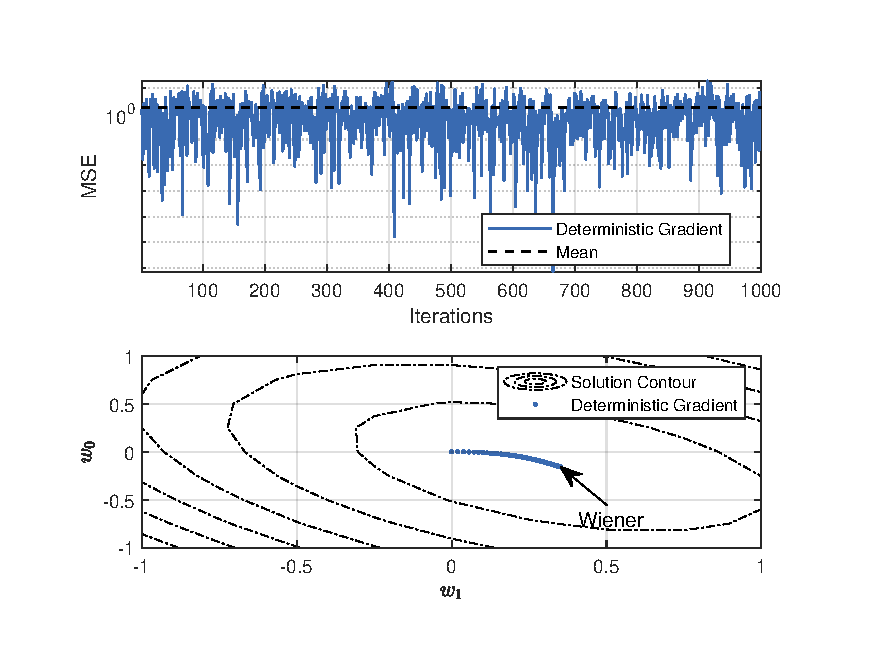
\includegraphics[width=0.80\textwidth]{fig/hw3p4-dga.pdf}
            \caption{Resultados da implementação do algoritmo gradiente determinístico com $N = 1000$ amostras, filtro de ordem $M = 2$ e parâmtro $\mu = 10^{-2}$. \textbf{Superior:} Evoulação da curva MSE. \textbf{Inferior:} Caminho percorrido até o ponto de convergência, i.e, filtro de Wiener.}
            \label{fig:hw3p4-dga}
        \end{figure}

        \begin{figure}[!htp]
            \centering
            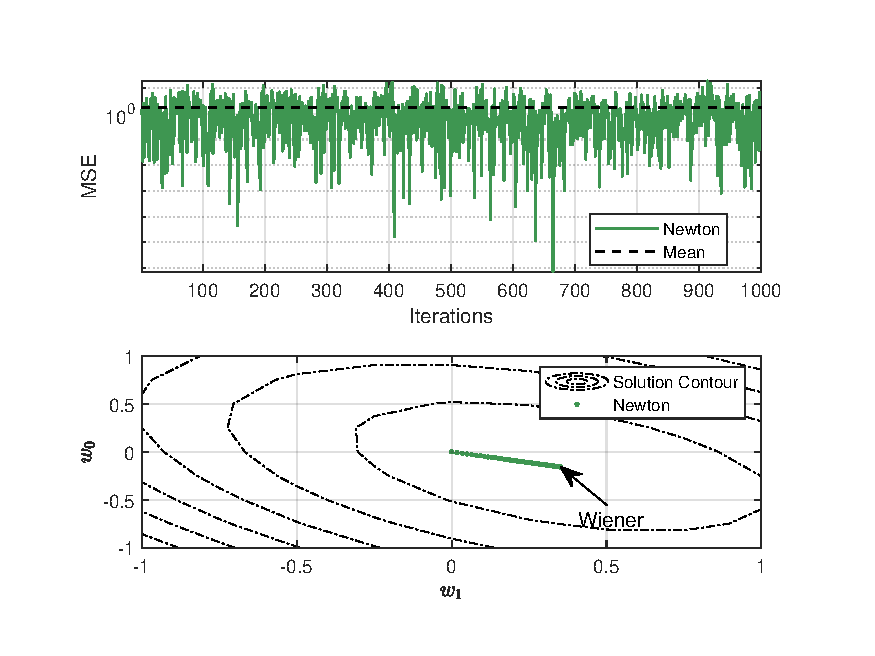
\includegraphics[width=0.80\textwidth]{fig/hw3p4-newton.pdf}
            \caption{Resultados da implementação do algoritmo Newton com $N = 1000$ amostras, filtro de ordem $M = 2$ e parâmtro $\mu = 0.5 \times 10^{-2}$. \textbf{Superior:} Evoulação da curva MSE. \textbf{Inferior:} Caminho percorrido até o ponto de convergência, i.e, filtro de Wiener.}
            \label{fig:hw3p4-newton}
        \end{figure}

        \begin{figure}[!htp]
            \centering
            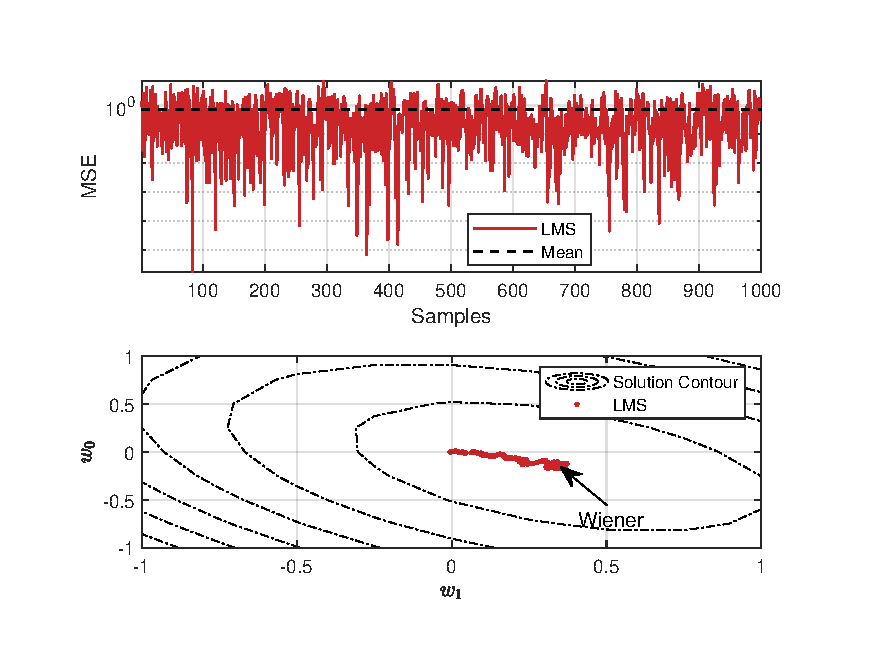
\includegraphics[width=0.80\textwidth]{fig/hw3p4-lms.pdf}
            \caption{Resultados da implementação do algoritmo LMS com $N = 1000$ amostras, filtro de ordem $M = 2$ e parâmtro $\mu = 10^{-3}$. \textbf{Superior:} Evoulação da curva MSE. \textbf{Inferior:} Caminho percorrido até o ponto de convergência, i.e, filtro de Wiener.}
            \label{fig:hw3p4-lms}
        \end{figure}

        \begin{figure}[!htp]
            \centering
            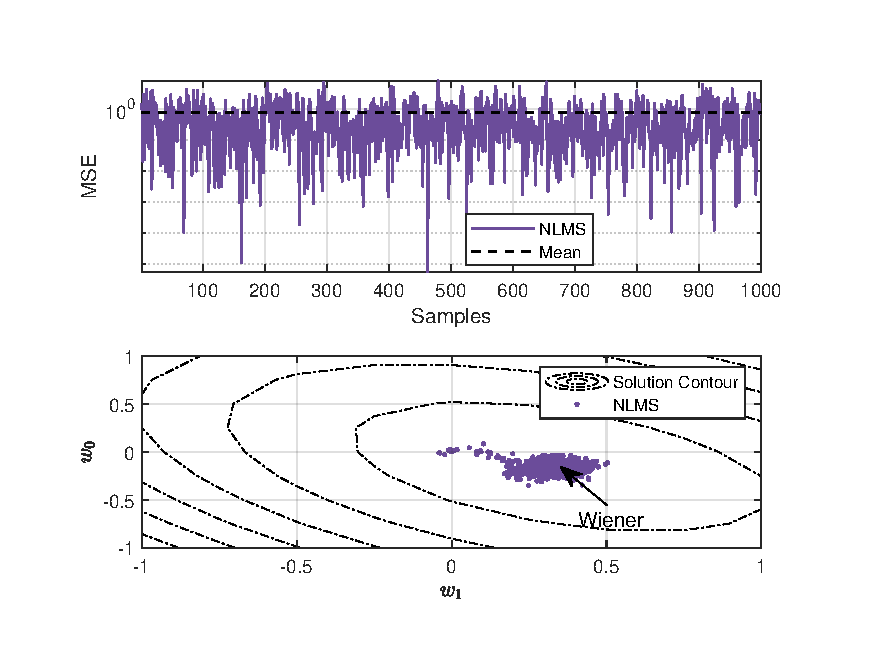
\includegraphics[width=0.80\textwidth]{fig/hw3p4-nlms.pdf}
            \caption{Resultados da implementação do algoritmo NLMS com $N = 1000$ amostras, filtro de ordem $M = 2$ e parâmtros $\mu = 0.5 \times 10^{-1}$ and $\gamma = 0.5 $. \textbf{Superior:} Evoulação da curva MSE. \textbf{Inferior:} Caminho percorrido até o ponto de convergência, i.e, filtro de Wiener.}
            \label{fig:hw3p4-nlms}
        \end{figure}

        
        \begin{figure}[!htp]
            \centering
            % \includegraphics[width=0.75\textwidth]{figs/newton_mse.png}
            \includegraphics[width=0.5\textwidth]{example-image}
            \caption{Evolução do MSE para o Método de Newton. $\text{Amostras} = 1000$, $M = 2$, $\mu = 10^{-3}$}
            \label{fig:newton_mse}
        \end{figure}
        
        \begin{figure}[!htp]
            \centering
            % \includegraphics[width=0.75\textwidth]{figs/gradient_mse.png}
            \includegraphics[width=0.5\textwidth]{example-image}
            \caption{Evolução do MSE para o Gradiente Determinístico. $\text{Amostras} = 1000$, $M = 2$, $\mu = 10^{-3}$}
            \label{fig:gradient_mse}
        \end{figure}
        
        \begin{figure}[!htp]
            \centering
            % \includegraphics[width=0.75\textwidth]{figs/lms_mse.png}
            \includegraphics[width=0.5\textwidth]{example-image}
            \caption{Evolução do MSE para o LMS. $\text{Amostras}  = 1000$, $M = 2$, $\mu = 10^{-3}$}
            \label{fig:lms_mse}
        \end{figure}

        \begin{figure}[!htp]
            \centering
            % \includegraphics[width=0.75\textwidth]{figs/nlms_mse.png}
            \includegraphics[width=0.5\textwidth]{example-image}
            \caption{Evolução do MSE para o NLMS. $\text{Amostras} = 1000$, $M = 2$, $\mu = 0.5$}
            \label{fig:nlms_mse}
        \end{figure}
        
        \begin{figure}[!htp]
            \centering
            % \includegraphics[width=0.75\textwidth]{figs/nlms_awgn.png}
            \includegraphics[width=0.5\textwidth]{example-image}
            \caption{Evolução do MSE para o NLMS em um Canal AWGN 30dB. $\text{Amostras} = 1000$, $M = 15$, $\mu = 0.5$}
            \label{fig:nlms_awgn}
        \end{figure}

\clearpage 

    \item Qual o número de condicionamento para o problema em questão?
    
        \textcolor{red}{Solução:}
        
        O número de condicionamento pode ser prontamente obtido pela expressão

        \begin{align}
            \mathbb{C} (\mathbf{R}_{x}) = \frac{\lambda_{\text{max}}}{\lambda_{\text{min}}},
        \end{align}
    
        onde $\lambda_{\text{max}}$ e $\lambda_{\text{min}}$ são os autovalores máximo e mínimo da matriz de autocorrelação, respectivamente. Por meio de um software
        matemático foi possível obter os seguinte autovalores para a matriz de autocorrelação teórica

        \begin{align}
            \mathbb{C} (\mathbf{R}_{x}) = \frac{5.16}{1.96} = 2.63,
        \end{align}

        onde talvez seja importante ressaltar que também poderiamos ter obtido os autovalores resolvendo a equação do polinômio
        característico da matriz de autocorrelação que é dada por

        \begin{align}
            \lambda^{2} - 7.12 \lambda + 10.11 = 0. 
        \end{align}

    \item Qual deveria ser o canal para que o número de condicionamento fosse menor/maior que 5?
    Comente os resultados.
    
        \textcolor{red}{Solução:}
        
        Inicialmente podemos escrever a matriz de correlação contabilizando a contribuição dos coeficientes do canal para os elementos individuais
        
        \begin{align}
            \mathbf{R}_{y} =
            \begin{bmatrix}
                a_{0} + a^{2}_{1} & a_{1}\\
                a_{1} & a_{0} + a^{2}_{1}
            \end{bmatrix},
        \end{align}

        onde a função de transferência do canal seria dada por $H(z) = a_{0} + a_{1}z^{-1}$. A partir dessa matriz de autocorrelação genérica podemos então 
        definir o seguinte polinômio característico

        \begin{align}
            &(\lambda - a_{0} + a^{2}_{1})^{2} - a^{2}_{1} = 0, \\
            &\lambda^{2} \underbrace{- 2 (a_{0} + a^{2}_{1})}_{b} \lambda + \underbrace{(a_{0} + a^{2}_{1})^{2} - a^{2}_{1}}_{c} = 0, \\
            &\lambda^{2} + b \lambda + c = 0,
        \end{align}

        onde sabemos que a solução é facilmente obtida pela fórmula de Bháskara. A partir disso podemos definir o número de condicionamento como

        \begin{align}
            \mathbb{C} (\mathbf{R}_{x}) &= \frac{\lambda_{\text{max}}}{\lambda_{\text{min}}}, \\
            \mathbb{C} (\mathbf{R}_{x}) &= \frac{- b + \sqrt{b^{2} - 4c}}{- b - \sqrt{b^{2} - 4c}}, \\
            \mathbb{C} (\mathbf{R}_{x}) &= \frac{2 (a_{0} + a^{2}_{1}) + \sqrt{4 (a_{0} + a^{2}_{1})^{2} - 4 (a_{0} + a^{2}_{1})^{2} + 4 a^{2}_{1}}}{2 (a_{0} + a^{2}_{1}) - \sqrt{4 (a_{0} + a^{2}_{1})^{2} - 4 (a_{0} + a^{2}_{1})^{2} + 4 a^{2}_{1}}}, \\
            \mathbb{C} (\mathbf{R}_{x}) &= \frac{2 (a_{0} + a^{2}_{1}) + 2a_{1}}{2 (a_{0} + a^{2}_{1}) - 2a_{1}}, \\
            \mathbb{C} (\mathbf{R}_{x}) &= \frac{a_{0} + a^{2}_{1} + a_{1}}{a_{0} + a^{2}_{1} - a_{1}},
        \end{align}

        assim temos agora uma fórmula para o número de condicionamento da matriz de autocorrelação com base nos coeficientes de canal. A partir disso basta que as seguintes inequações sejam atendidas para que
        obtenhamos um número de condicionamento maior ou menor do que o requerido

        \begin{align}
            a_{0} + a^{2}_{1} + a_{1} &\geq 5 (a_{0} + a^{2}_{1} - a_{1}), \\
            a_{0} + a^{2}_{1} + a_{1} &\leq 5 (a_{0} + a^{2}_{1} - a_{1}).
        \end{align}

\end{enumerate}


\clearpage


\subsection{Identificação de Sistemas} % <-----------------------------------------------------------------------------
\todo[inline, color=yellow!30]{Organizar}

    
\begin{align}
    H(z) = \frac{1 - z^{-12}}{1 - z^{-1}}
\end{align}

\begin{enumerate}

    \item Calcule o limite superior para $\mu$ (ou seja $\mu_{\text{max}}$) para garantir a estabilidade do algoritmo.

        \textcolor{red}{Solução:}

        Para garantirmos a estabilidade do algoritmo precisamos apenas obter o valor numérico do maior autovalor definido pela matriz de autocorrelação do problema.
        Desse modo, podemos simplificar a função de transferência por meio da seguinte manipulação algébrica

        \begin{align*}
            H(z) &= \frac{1 - z^{-12}}{1 - z^{-1}}, \\
            H(z) &= \frac{(1 - z^{-1})(1 + z^{-1} + z^{-2} + z^{-3} + z^{-4} + z^{-5} + z^{-6} + z^{-7} + z^{-8} + z^{-9} + z^{-10} + z^{-11})}{1 - z^{-1}}, \\
            H(z) &= 1 + z^{-1} + z^{-2} + z^{-3} + z^{-4} + z^{-5} + z^{-6} + z^{-7} + z^{-8} + z^{-9} + z^{-10} + z^{-11},
        \end{align*}

        e tomando a transformada z inversa da função de transferência chega-se a seguinte saída de um sinal transmitido por esse canal

        \begin{align*}
            y(n) &= x(n) + x(n-1) + x(n-2) + x(n-3) + x(n-4) + x(n-5) + x(n-6) + x(n-7) \\
            &+ x(n-8) + x(n-9) + x(n-10) - x(n-11), 
        \end{align*}

        Em sequência é possível utilizar um software matemático para obter uma estimação para a matriz de autocorrelação

        \begin{figure}[!htp]
            \centering
            % \includegraphics[width=1\textwidth]{figs/Rxx.png}
            \includegraphics[width=0.3\textwidth]{example-grid-100x100pt}
        \caption{Matriz de autocorrelação estimada após 10000 realizações para retirada do comportamento médio}
        \label{fig:rxx}
        \end{figure}

        onde a análise de autovalores de $\mathbf{R}_{xx}$ resulta no seguinte intervalo de convergência para o passo de 
        aprendizado

        \begin{align}
            0 < \mu < \frac{1}{\lambda_{\text{max}}} = \frac{1}{97} \approx 0.01,
        \end{align}

        e assim $\mu_{\text{max}} \approx 0.01$.

    \item Execute o algoritmo para $\frac{\mu_{\text{max}}}{2}$, $\frac{\mu_{\text{max}}}{10}$ e $\frac{\mu_{\text{max}}}{50}$. Comente sobre o comportamento da convergência de cada caso.

        \textcolor{red}{Solução:}


        Nas Figuras \ref{fig:mu_2}, \ref{fig:mu_10} e \ref{fig:mu_50} podemos verificar o comportamento da convergência do algoritmo para esse problema. A príncipio é possível 
        confirmar que existe uma diminuta piora quanto ao desempenho dos algoritmos a medida que o passo de aprendizado descrece. Isso pode ser explicado pois a medida que 
        $\mu$ fica menor a flexibilidade de adaptação do algoritmo é reduzida. Assim, para passos de aprendizado muito pequenos é mais difícil para o filtro conseguir acompanhar
        as mudanças no canal provocadas pelo impacto de componentes ruidosas e pela resposta em frequência do canal. 

        \begin{figure}[!htp]
            \centering
            % \includegraphics[width=0.75\textwidth]{figs/L3Q5_mu_2.png}
            \includegraphics[width=0.5\textwidth]{example-image}
            \caption{$\text{Amostras} = 1000$, $M = 15$, $\mu = \frac{\mu_{\text{max}}}{2}$}
            \label{fig:mu_2}
        \end{figure}
    
        \begin{figure}[!htp]
            \centering
            % \includegraphics[width=0.75\textwidth]{figs/L3Q5_mu_10.png}
            \includegraphics[width=0.5\textwidth]{example-image}
            \caption{$\text{Amostras} = 1000$, $M = 15$, $\mu = \frac{\mu_{\text{max}}}{10}$}
            \label{fig:mu_10}
        \end{figure}
    
        \begin{figure}[!htp]
            \centering
            % \includegraphics[width=0.75\textwidth]{figs/L3Q5_mu_50.png}
            \includegraphics[width=0.5\textwidth]{example-image}
            \caption{$\text{Amostras} = 1000$, $M = 15$, $\mu = \frac{\mu_{\text{max}}}{50}$}
            \label{fig:mu_50}
        \end{figure}
        
        \clearpage


        \item Meça o desajuste (misadjustment) em cada exemplo e comparar com os resultados obtidos pela solução teórica (Eq. (3.50) do livro texto)					

        \textcolor{red}{Solução:}

        O desajuste pode ser aproximado por

        \begin{align}
            M = \frac{\xi_{\text{excesso}}}{\xi_{\text{min}}} &\approx \frac{\mu \text{tr}(\mathbf{R}_{x})}{1 - \mu \text{tr}(\mathbf{R}_{x})},
        \end{align}

        e a partir dessa expressão foi possivel obter a seguinte tabela

        \begin{table}[!htp]
            \centering
            \begin{tabular}{|l|l|l|}
                \hline
                & Empírico & Téorico \\ \hline
                $\frac{\mu_{\text{max}}}{2}$  & $ -1.3865 $ &  $ -1.3846 $ \\ \hline
                $\frac{\mu_{\text{max}}}{10}$ & $ +2.5392 $ & $ +2.5714 $ \\ \hline
                $\frac{\mu_{\text{max}}}{50}$ & $ +0.1675 $ & $ +0.1682 $ \\ \hline
            \end{tabular}
        \end{table}

        Os resultados foram obtidos por uso de software matemático e os códigos estão disponíveis juntamente com este relatório.

    \item Mostre o gráfico da resposta em frequência do filtro FIR em qualquer uma das iterações após a convergência ser obtida e compare com o sistema desconhecido.

        \textcolor{red}{Solução:}

        A resposta em frequência do filtro está disponível nas Figuras \ref{fig:filter_response_2}, \ref{fig:filter_response_10} e \ref{fig:filter_response_50} para os casos $\frac{\mu_{\text{max}}}{2}$, $\frac{\mu_{\text{max}}}{10}$ e $\frac{\mu_{\text{max}}}{50}$, respectivamente. 
        É possível ver que a resposta em frequência do filtro tende a se aproximar da resposta em frequência do sistema quanto maior o passo de aprendizado, pois quanto maior $\mu$ mais facilidade tem o filtro em acompanhar as variações do canal. 
        No caso extremo onde temos um passo de aprendizado $\frac{\mu_{\text{max}}}{50}$ é possível verificar que a resposta em frequência do filtro é uma versão consideravelmente amortecida da resposta original do canal. 
        Ademais, na Figura \ref{fig:L3Q5_t} vemos a evolução temporal do filtro para as primeiras 100 amostras quando temos a resposta em frequência dada na Figura \ref{fig:filter_response_2}.

\end{enumerate}



\begin{figure}[!htp]
    \centering
    % \includegraphics[width=0.75\textwidth]{figs/L3Q5_filter_response_2.png}
    \includegraphics[width=0.5\textwidth]{example-image}
    \caption{$\text{Amostras} = 1000$, $M = 15$, $\mu = \frac{\mu_{\text{max}}}{2}$}
    \label{fig:filter_response_2}
\end{figure}

\begin{figure}[!htp]
    \centering
    % \includegraphics[width=0.75\textwidth]{figs/L3Q5_filter_response_10.png}
    \includegraphics[width=0.5\textwidth]{example-image}
    \caption{$\text{Amostras} = 1000$, $M = 15$, $\mu = \frac{\mu_{\text{max}}}{10}$}
    \label{fig:filter_response_10}
\end{figure}

\begin{figure}[!htp]
    \centering
    % \includegraphics[width=0.75\textwidth]{figs/L3Q5_filter_response_50.png}
    \includegraphics[width=0.5\textwidth]{example-image}
    \caption{$\text{Amostras} = 1000$, $M = 15$, $\mu = \frac{\mu_{\text{max}}}{50}$}
    \label{fig:L3Q5_t}
\end{figure}

\begin{figure}[!htp]
    \centering
    % \includegraphics[width=0.75\textwidth]{figs/L3Q5_t.png}
    \includegraphics[width=0.5\textwidth]{example-image}
    \caption{$\text{Amostras} = 1000$, $M = 15$, $\mu = \frac{\mu_{\text{max}}}{2}$}
    \label{fig:filter_response_50}
\end{figure}


\subsection{Equalização Adaptativa} % <-----------------------------------------------------------------------------
\todo[inline, color=yellow!30]{Organizar}

    
\begin{align}
    H(z) = 0.5 + 1.2z^{-1} + 1.5z^{-2} + z^{-3},
\end{align}

e deseja-se projetar um equalizar para o mesmo. A estrutura do equalizador é mostrada na Figura abaixo. Os símbolos $s(n)$ são transmitidos através de um canal e corrompidos por ruído aditivo gaussiano branco complexo $v(n)$. O sinal recebido $x(n)$ é processado pelo equalizador FIR para gerar estimativas $\overset{\sim}{s}(n - \delta)$, as quais são passados por um dispositivo decisor gerando  símbolos $\hat{s}(n - \delta)$. O equalizador possui dois modos de operação: um modo de treinamento durante o qual uma versão atrasada e  replicada da sequência de entrada é usada como o sinal de referência (desejado) e um modo dirigido por decisão no qual a saída do dispositivo de decisão substitui a sequência de referência. O sinal de entrada $s(n)$ é escolhido de uma constelação QAM (por exemplo, 4-QAM, 16-QAM, 64-QAM ou 256-QAM).



\begin{enumerate}
    
    \item Faça um programa que treine o filtro adaptativo com 500 símbolos de uma constelação 4-QAM, seguindo de uma operação dirigida por decisão de 5000 símbolos de uma constelação 16-QAM. Escolha a variância do ruído $\sigma^{2}_{v}$ de maneira que ela promova uma relação sinal ruído de 30 db na entrada do equalizador. Note que os símbolos escolhidos não têm variância unitária. Por esta razão, a a variância do ruído necessita ser ajustada adequadamente para cada uma das diferentes modulações (constelações) QAM para fornecer o nível de SNR desejado. Escolha $\delta = 15$ e o comprimento do equalizador M = 15. Mostre os gráficos da evolução temporal de $s(n)$, $x(n)$ e $\overset{\sim}{s}(n - \delta)$. Use o LMS-normalizado com um fator de passo de $\mu = 0.4$.
                
        \textcolor{red}{Solução:}

        Os resultados estão nas Figuras \ref{fig:L3Q6A1} e \ref{fig:L3Q6A2}. A evolução temporal do MSE apresenta comportamento similar aos resultados apresentados anteriormente com
        o MSE possuindo uma grande variação mesmo após a convergência. Por fim, também é possível ver na figura seguinte o impacto no filtro na filtragem de um sinal modulado por 16-QAM. É visível 
        que a estimação conseguiu separar o sinal transmitido em diferentes regiões de decisão e assim seria necessário ao fim desse processo passar esse sinal filtrado por um decisor para que fosse
        obtida uma aproximação do sinal originalmente trnasmitido. Ademais, foi implementado um simples processo de aprendizado utilizando algumas amostras de sinais 4-QAM para o treinamento do filtro com
        o objetivo de facilitar ou acelerar a convergência quando o sinal 16-QAM fosse filtrado. 
        
        Além disso, na Figura \ref{fig:L3Q6A3} é possível acompanhar a evolução temporal do sinal filtrado e do sinal 
        original para dois momentos distintos. No primeiro, temos a adaptação do filtro para as primeiras 100 amostras e previsivelmente confirmamos que o filtro possuí ainda dificuldades em acompanhar o canal 
        nas primeiras amostras. Já no segundo momento temos as últimas 100 amostras do filtro e podemos entender a partir disso que o filtro agora tem capacidade de acompanhar o canal de forma mais eficiente, embora
        ainda existam momentos onde erros ocorrem. Esses erros podem ser ocasionados pelas interferências ruidosas que provocam erros de detecção na hora de avaliar as constelações aproximadas que saem do processo de filtragem.

        \begin{figure}[!htp]
            \centering
            % \includegraphics[width=0.75\textwidth]{figs/L3Q6_A_mse.png}
            \includegraphics[width=0.5\textwidth]{example-image}
            \caption{$\text{Amostras} = 5000$, $M = 15$, $\mu = 0.4$}
            \label{fig:L3Q6A1}
        \end{figure}
        
        \begin{figure}[!htp]
            \centering
            % \includegraphics[width=0.75\textwidth]{figs/L3Q6_A_c.png}
            \includegraphics[width=0.5\textwidth]{example-image}
            \caption{$\text{Amostras} = 5000$, $M = 15$, $\mu = 0.4$}
            \label{fig:L3Q6A2}
        \end{figure}
        
        \begin{figure}[!htp]
            \centering
            % \includegraphics[width=0.75\textwidth]{figs/L3Q6_A_t.png}
            \includegraphics[width=0.5\textwidth]{example-image}
            \caption{$\text{Amostras} = 5000$, $M = 15$, $\mu = 0.4$}
            \label{fig:L3Q6A3}
        \end{figure}
        
        \clearpage

    \item Para os mesmos parâmetros do item (a), plote e compare os gráficos de evolução que seriam resultante se o equalizador fosse treinado com 150, 300 e 500 iterações. Use o LMS com um
    $\mu = 0.001$.
    
        \textcolor{red}{Solução:}

        O resultado está na Figura \ref{fig:L3Q6B}. Particularmente não pude distinguir notáveis diferenças de desempenho ao considerar diferentes tamanhos de sequências de treinamento.

            
    \begin{figure}[!htp]
        \centering
        % \includegraphics[width=0.75\textwidth]{figs/L3Q6_B_t.png}
        \includegraphics[width=0.5\textwidth]{example-image}
        \caption{$\text{Amostras} = 5000$, $M = 15$, $\mu = 0.001$}
        \label{fig:L3Q6B}
    \end{figure}

    \item Assuma agora que os dados transmitidos foram gerados de uma constelação 256-QAM ao invés de 16-QAM. Plote os gráficos da evolução do sinal na saída do equalizador quando treinado
    usando o LMS-normalizado e 500 símbolos de treinamento.					
    
        \textcolor{red}{Solução:}

        Os resultados estão nas Figuras \ref{fig:L3Q6C1} e \ref{fig:L3Q6C2}. É possível verificar na primeira figura que a evolução do MSE aconteceu apesar de uma considerável variação ao final
        da convergência. Já em relação a figura seguinte, onde transmitimos um sinal 256-QAM e utilizamos um filtro treinado por um sinal 4-QAM, é possível verificar que inicialmente o filtro demonstrou dificuldade em acompanhar
        a evolução do canal. Por fim, em um segundo momento é apresentado a evolução temporal considerando as ultimas amostras do sinal e aqui podemos visualizar que, embora ainda existam uma quantidade considerável de erros por se 
        tratar de uma modulação de ordem elevada, o filtro consegue se aproximar com um pouco mais de facilidade do sinal original. 
        
        Adicionalmente, para termos uma melhor interpretação do desempenho desse filtro seria necessário utilizar 
        uma métrica como a SER ou BER e comparar o impacto de diferentes modulações no desempenho do algoritmo de filtragem. Isso se deve pois quando utilizamos um decisor o símbolo filtrado pode ser alocado para uma região da constelação
        da modulação a qual não pertence. Entretanto, tais erros de decisão so são aparente quando utilizamos uma métrica capaz de capturar tal fenômeno.
        
        
    \begin{figure}[!htp]
        \centering
        % \includegraphics[width=0.75\textwidth]{figs/L3Q6_C_mse.png}
        \includegraphics[width=0.5\textwidth]{example-image}
        \caption{$\text{Amostras} = 5000$, $M = 15$, $\mu = 0.4$}
        \label{fig:L3Q6C1}
    \end{figure}

    \begin{figure}[!htp]
        \centering
        % \includegraphics[width=0.75\textwidth]{figs/L3Q6_C_t.png}
        \includegraphics[width=0.5\textwidth]{example-image}
        \caption{$\text{Amostras} = 5000$, $M = 15$, $\mu = 0.4$}
        \label{fig:L3Q6C2}
    \end{figure}

    \item Gerar as curvas de taxa de erro de símbolo (SER, do inglês Symbol Error Rate) versus SNR na entrada do equalizador para símbolos de constelações 4, 16, 64 e 256-QAM. Faça SNR variar
    de 5dB a 30dB.
    
        \textcolor{red}{Solução:}

        Os resultados estão na Figura \ref{fig:L3Q6D}. Assim, podemos analisar o real desempenho do filtro quando associado a um equalizador que desconhece o sinal verdadeiro. 
        É possível verificar que a medida que a ordem de modulação aumenta o desempenho sofre uma considerável piora. Existem duas principais razões para explicar esse comportamento. A primeira vem justamente 
        do tamanho das constelações digitais que a medida que a ordem aumenta tem uma menor regiao de decisão associada aos seus símbolos. Desse modo, o sinal transmitido fica sujeito a interferências de componentes 
        ruidosas do canal pois as divisórias entre as diversas regiões de decisão dos símbolos da modulação ficam menores e erros de decisão irão acontecer com maior frequência A segunda razão poderia ser explicada pelo 
        fato do filtro ter sido inicialmente treinado utilizando símbolos modulados com 4-QAM, mas provavelmente isso é insuficiente quando a ordem de modulação do sinal transmitido cresce.
        Ademais, vale ressaltar que não houve erros para SNR $= 30$ dB quando se transmitiu sinais 4-QAM, entretanto como foram utilizados apenas 1000 realizações de Monte Carlo não foi
        possível capturar erros para esse ponto específico de SNR.

        
    \begin{figure}[!htp]
        \centering
        % \includegraphics[width=0.75\textwidth]{figs/L3Q6_D_ser.png}
        \includegraphics[width=0.5\textwidth]{example-image}
        \caption{$\text{Amostras} = 5000$, $M = 15$, $\mu = 0.4$}
        \label{fig:L3Q6D}
    \end{figure}


\end{enumerate}
